\section{Changes in demand risk exposure}
Trading volume is difficult to define because it depends on the asset structure. Therefore, we introduce a measure that is independent of the asset structure but nevertheless captures the effects of disagreement on trading volume with the caveat that is not directly comparable to trade in a specific asset. Specifically, Definition \ref{Def:TotExpsure} below introduces the concept of excess exposure to supply and demand shocks. It basically captures how investors' optimal portfolios deviate from two-fund separation. Based on this measure, we define trading volume as variations of excess exposure and determine it in Proposition \ref{prop:TradingVolume} below. This measure captures the notion that large changes in excess exposure have to come from changes in underlying asset positions. 

 \begin{defn}[Excess Exposure]\label{Def:TotExpsure}
 Let $\mu^{W,i}_{s,t}$ denote the drift, $\sigma^{W,i}_{Y,s,t}$ the supply shock (output) exposure, and $\sigma^{W,i}_{\alpha,s,t}$ the demand shock exposure of a patient (type i=a) and impatient (type i=b) investor born at time $s$ with total wealth dynamics
 \begin{equation} \label{eq:totwealthind}
 \frac{dW^i_{s,t}}{W^i_{s,t}} = \mu^{W,i}_{s,t} \:  dt + \sigma^{W,i}_{Y,s,t} \: dZ_{Y,t}  
	+ \sigma^{W,i}_{\alpha,s,t} \: dZ_{\alpha,t}.
\end{equation}
Investors' supply and demand shock exposure in excess of their exposure to both shocks trough the value of their endowment stream is defined as 
\begin{align}\label{eq:XE_Y}
   \text{XE}_{Y,t} &= \int_{-\infty}^{t} \nu e^{\nu \left(t-s\right)}\left(\alpha_s \beta^{W,a}_{s,t} \lvert  \sigma^{W,a}_{Y,s,t} \rvert 
 +\left(1-\alpha_s\right) \beta^{W,b}_{s,t} \lvert \sigma^{W,b}_{Y,s,t}  \rvert \right)ds  -  \lvert \sigma^{Y}_{R,t}\rvert \\
  \text{XE}_{\alpha,t} &= \int_{-\infty}^{t} \nu e^{\nu \left(t-s\right)}\left(\alpha_s \beta^{W,a}_{s,t}  \lvert \sigma^{W,a}_{\alpha,s,t} \rvert 
 +\left(1-\alpha_s\right)\beta^{W,b}_{s,t} \lvert  \sigma^{W,b}_{\alpha,s,t}  \rvert \right)ds -  \lvert \sigma^{\alpha}_{R,t}\rvert,
\end{align} 
respectively, where $\beta^{W,i}_{s,t} =  W^i_{s,t}/ W_t$ denotes the individual wealth share of a type i investor. 
\end{defn}
We derive the excess exposure to supply and demand shocks in the next proposition.
\begin{prop}[Excess Exposure]\label{prop:Exposure}
 The individual supply shock exposure, demand shock exposure, and drift of investors' wealth $W^i_{s,t}$ is $ \sigma^{W,i}_{Y,s,t} = \sigma_Y$,  $\sigma^{W,i}_{\alpha,s,t} = \theta_{\alpha,t}^i$, and $\mu^{W,i}_{s,t} =  r_t +\sigma_Y^2+\left( \theta_{\alpha,t}^i \right)^2 -\rho^i$, respectively. 
There is no excess exposure to supply shocks, that is,  is $\text{XE}_{Y,t} =0$ but there is excess exposure to demand shocks. Specifically,
 \begin{equation}\label{eq:XEdemand}
	\text{XE}_{\alpha,t}= 2 \frac{\phi_b}{\phi_t}  f_t  \left(1-f_t\right) \Delta = 2 \frac{\phi_b}{\phi_a-\phi_b} \sigma^{\alpha}_{R,t} \geq 0. 
\end{equation}
\end{prop} 
There is no disagreement on supply shocks and consequently investors do not speculate on it. Hence, investors' fractions of wealth invested in the market portfolio are equally exposed to supply shocks and, thus, there is no excess exposure to these shocks. If investors disagree on demand shocks, then they trade on this disagreement and by doing so invest different fractions of their wealth in the market portfolio even though they have the same risk preferences. The more they deviate from two-fund separation, the larger the excess exposure to demand shocks.   Equation (\ref{eq:XEdemand}) shows that this exposure is  proportional to the stock market loading onto demand shocks and, thus, inherits all properties of the stock market volatility. 

We define trading volume or trading intensity as the square root of the instantaneous quadratic variation of excess exposure to demand shocks. This is similar to the continuous time literature that typically use the quadratic variation of portfolio policies as a measure of the trading intensity (e.g. \cite{grossman-zhou:96}, \cite{longstaff-wang:12}, and \cite{EhlingHeyerdahlLarsen2016}).  

\begin{prop}\label{prop:TradingVolume}
 Let $QV_{t,T}$ denote the quadratic variation of excess demand risk exposure. Specifically,
 \begin{equation}
  QV_{t,T} = \int_t^{T} d\text{XE}_{\alpha,u} d\text{XE}_{\alpha,u} = \int_t^{T} \left(\text{TVol}_u\right)^2 \: du.
 \end{equation}
 Then $\text{TVol}_t$ denotes the trading volume or trading intensity. Specifically, 
\begin{equation}\label{eq:TVol}
	\text{TVol}_t = 2\phi^b \Delta^2  \frac{f_t (1-f_t) }{\phi_t^2} \lvert \phi^B \left(1-f_t\right)^2 - \phi^A f_t^2   \rvert.
\end{equation}
\end{prop}

\begin{figure}[H] 
\centering
\begin{tabular}{cc}
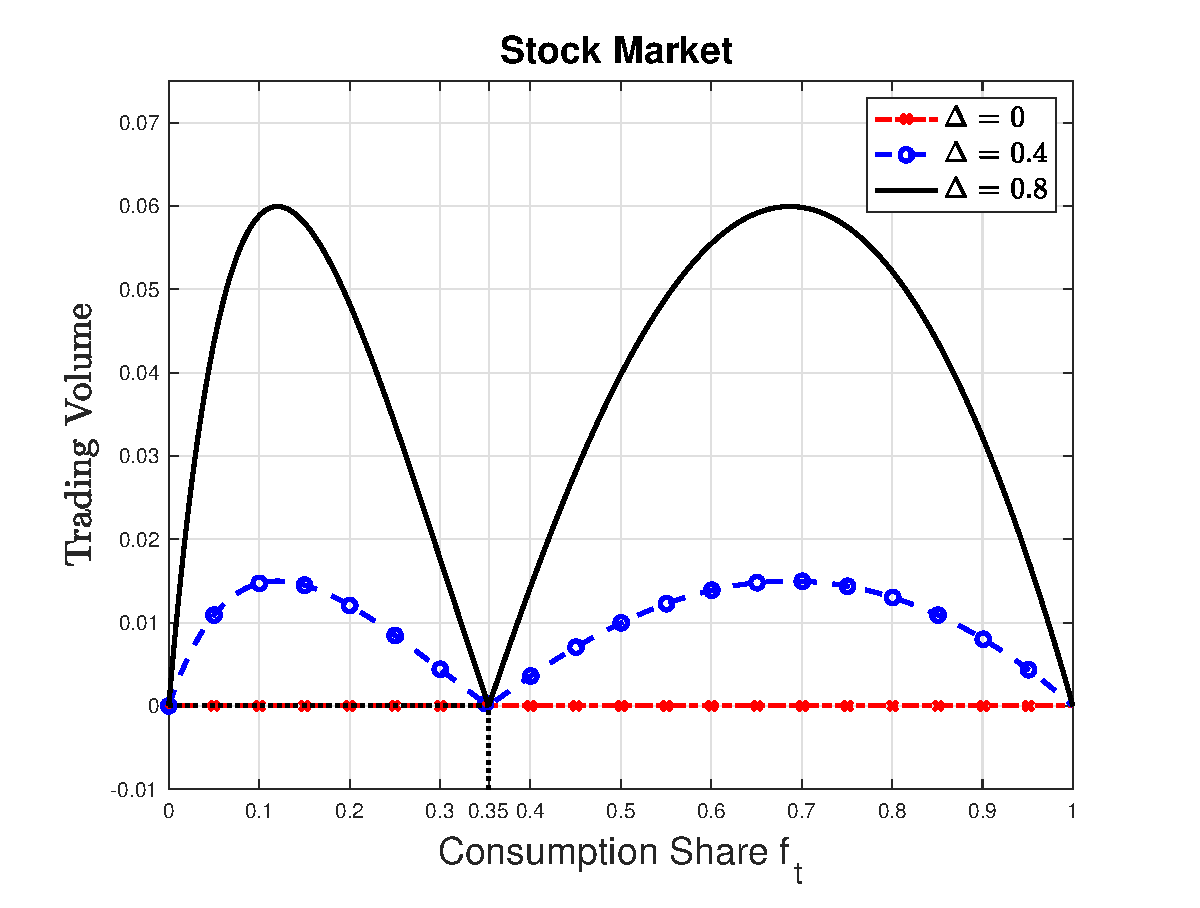
\includegraphics[width=.4\textwidth]{figures/TradingVolume2f.eps} &
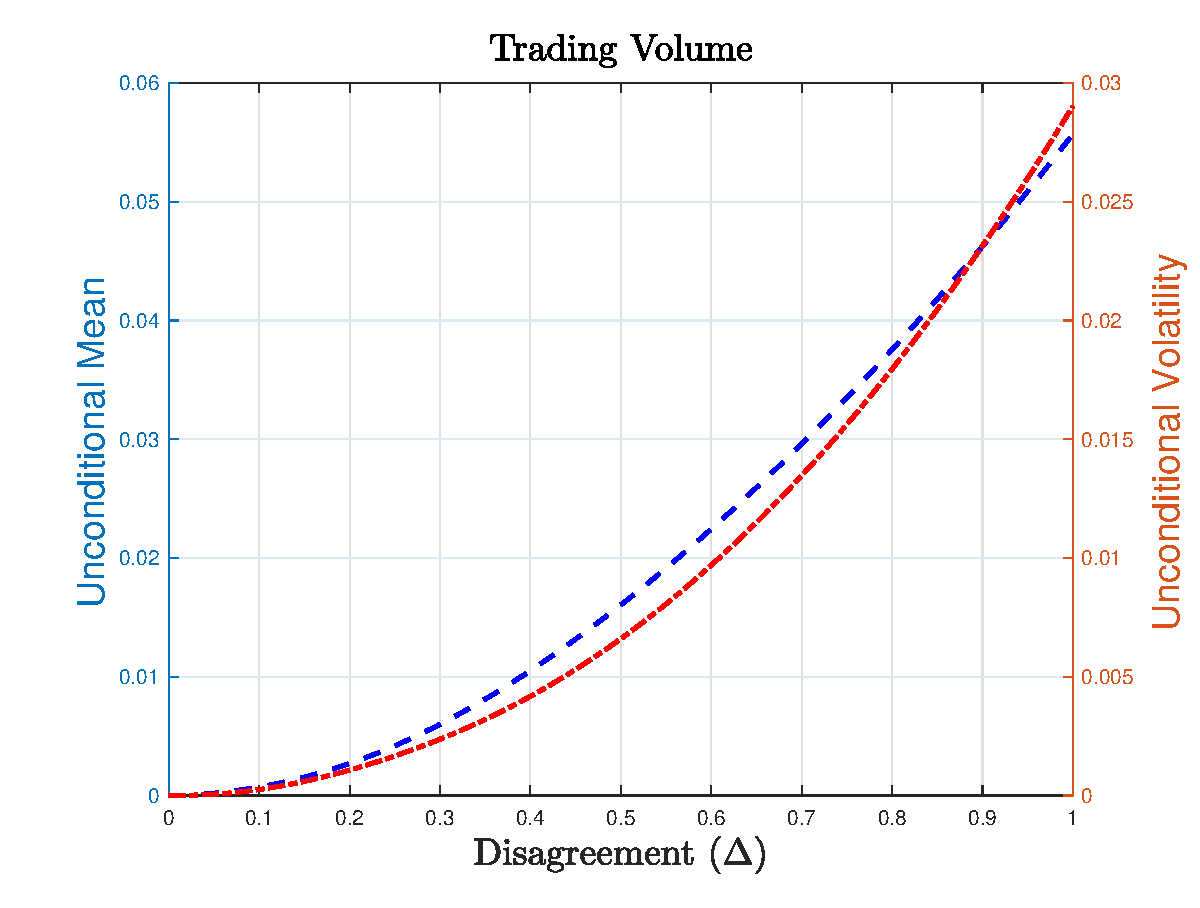
\includegraphics[width=.4\textwidth]{figures/TradingVolume2DELmeanvol.eps} 
\end{tabular}
\caption{\emph{Trading volume or trading intensity.} \footnotesize{The left graph shows trading volume/intensity as a function of the consumption share $f_t$ for different disagreement $\Delta$ and the right graph shows the unconditional mean and volatility of it as a function of disagreement $\Delta$. Trading volume is a non monotone function of the consumption share but both its mean and volatility are strictly increasing in disagreement. The unconditional statistics are based on one million years of monthly observations. In this example the parameters are based on the alternative calibration with $\rho^a = 0.001$ and $\rho^b = 0.05$}}   \label{fig:tradingf} 
\end{figure}

The left graph of Figure \ref{fig:tradingf} shows that trading volume is a non monotone function of the consumption share that is increasing in disagreement. Moreover, the right graph of Figure \ref{fig:tradingf} shows that the unconditional mean and volatility of trading volume is strictly increasing in disagreement. 
